% Copyright 2004 by Till Tantau <tantau@users.sourceforge.net>.
%
% In principle, this file can be redistributed and/or modified under
% the terms of the GNU Public License, version 2.
%
% However, this file is supposed to be a template to be modified
% for your own needs. For this reason, if you use this file as a
% template and not specifically distribute it as part of a another
% package/program, I grant the extra permission to freely copy and
% modify this file as you see fit and even to delete this copyright
% notice. 

\documentclass{beamer}

% There are many different themes available for Beamer. A comprehensive
% list with examples is given here:
% http://deic.uab.es/~iblanes/beamer_gallery/index_by_theme.html
% You can uncomment the themes below if you would like to use a different
% one:
%\usetheme{AnnArbor}
%\usetheme{Antibes}
%\usetheme{Bergen}
%\usetheme{Berkeley}
%\usetheme{Berlin}
%\usetheme{Boadilla}
%\usetheme{boxes}
%\usetheme{CambridgeUS}
%\usetheme{Copenhagen}
%\usetheme{Darmstadt}
\usetheme{default}
\usepackage[utf8x]{inputenc}
%\usetheme{Frankfurt}
%\usetheme{Goettingen}
%\usetheme{Hannover}
%\usetheme{Ilmenau}
%\usetheme{JuanLesPins}
%\usetheme{Luebeck}
%\usetheme{Madrid}
%\usetheme{Malmoe}
%\usetheme{Marburg}
%\usetheme{Montpellier}
%\usetheme{PaloAlto}
%\usetheme{Pittsburgh}
%\usetheme{Rochester}
%\usetheme{Singapore}
%\usetheme{Szeged}
%\usetheme{Warsaw}

\usepackage{listings}
\usepackage{color}

\definecolor{dkgreen}{rgb}{0,0.6,0}
\definecolor{gray}{rgb}{0.5,0.5,0.5}
\definecolor{mauve}{rgb}{0.58,0,0.82}

\lstset{frame=tb,
  language=PHP,
  aboveskip=3mm,
  belowskip=3mm,
  showstringspaces=false,
  columns=flexible,
  basicstyle={\footnotesize\ttfamily},
  numbers=none,
  numberstyle=\tiny\color{gray},
  keywordstyle=\color{blue},
  commentstyle=\color{dkgreen},
  stringstyle=\color{mauve},
  breaklines=true,
  breakatwhitespace=true,
  tabsize=3
}


\title{PHP/MySQL development}

% A subtitle is optional and this may be deleted
\subtitle{a Twitter-like application}

\author{Maxime Martineau}
% - Give the names in the same order as the appear in the paper.
% - Use the \inst{?} command only if the authors have different
%   affiliation.

\institute[Polytech Tours] % (optional, but mostly needed)
{
    Polytech Tours Département Informatique  
}
% - Use the \inst command only if there are several affiliations.
% - Keep it simple, no one is interested in your street address.

\date{\today}
% - Either use conference name or its abbreviation.
% - Not really informative to the audience, more for people (including
%   yourself) who are reading the slides online

\subject{Database}
% This is only inserted into the PDF information catalog. Can be left
% out. 

% If you have a file called "university-logo-filename.xxx", where xxx
% is a graphic format that can be processed by latex or pdflatex,
% resp., then you can add a logo as follows:

% \pgfdeclareimage[height=0.5cm]{university-logo}{university-logo-filename}
% \logo{\pgfuseimage{university-logo}}

% Delete this, if you do not want the table of contents to pop up at
% the beginning of each subsection:
\AtBeginSubsection[]
{
  \begin{frame}<beamer>{Outline}
    \tableofcontents[currentsection,currentsubsection]
  \end{frame}
}

% Let's get started
\begin{document}

\begin{frame}
  \titlepage
\end{frame}

\begin{frame}{Outline}
    \tableofcontents
\end{frame}

\section{The project}
\begin{frame}
    Twitter application
    
    \begin{itemize}
        \item Users : can post, follow a user, …
        \item Post : message from a user
        \item Notification system
        \item Hashtag : to mark a given topic (ex: \#DevelopersBeLike)
    \end{itemize}
\end{frame}

\begin{frame}{Frame}
\begin{itemize}
\item 6 practical works (12h)
\item Work in pairs
\item Code to give back at the end (the database schema in \texttt{db/} + the \texttt{model/} files)
\end{itemize}
\end{frame}

\begin{frame}{Project structure}
\center
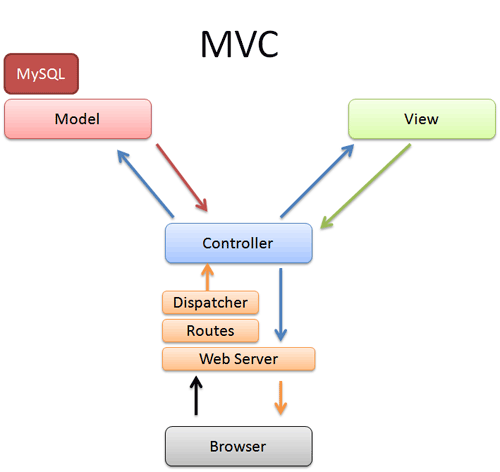
\includegraphics[scale=0.3]{images/mvc-rails.png}
\end{frame}

\section{PHP}

\begin{frame}[fragile]{PHP : Data}
    \begin{itemize}
        \item Declare a variable
        \begin{lstlisting}
$a = 23; // $a is an int
$b = 2.3; // $b is a float
$c = true; // $c is a boolean
$d = array("a", 1, "b"); // $d is an array
        \end{lstlisting}
    \end{itemize}
\end{frame}

\begin{frame}[fragile]{PHP: Data}
    \begin{itemize}
        \item Deal with arrays
        \begin{lstlisting}
$a = array("a", "b", 1);
echo $a[0]; // prints "a"
$a[0] = "A";
echo $a[0]; // ?
$a[] = 2; // $a == ?
        \end{lstlisting}
        \item Associative arrays
        \begin{lstlisting}
$fruit = array("name" => "strawberry", "color" => "red");
echo $fruit["name"]; // ?
echo $fruit["color"]; // ?
$fruit["color"] = "black";
        \end{lstlisting}
    \end{itemize}
\end{frame}

\begin{frame}[fragile]{PHP : Data}
    \begin{itemize}
        \item Create and use a stdClass object
        \begin{lstlisting}
$fruit = (object) array("name" => "strawberry", "color" => "red");
echo $fruit->name; // ?
echo $fruit->color; // ?
        \end{lstlisting}
    \end{itemize}
\end{frame}

\begin{frame}[fragile]{PHP : Controls}
    \begin{itemize}
        \item If stanzas
        \begin{lstlisting}
if($a == 1) {
    echo "yoohoo :D";
}
else {
    echo "oh :(";
}

        \end{lstlisting}
    \end{itemize}
\end{frame}

\begin{frame}[fragile]{PHP : Controls}
    \begin{itemize}
        \item While loops
        \begin{lstlisting}
$i = 0;
while($i <= 10) {
    echo $i;
    $i++;
}
        \end{lstlisting}
        \item For loops
        \begin{lstlisting}
for($i = 0; $i <= 10; $i++) {
    echo $i;
}
        \end{lstlisting}
        \item Foreach loops
        \begin{lstlisting}
$arr = array(0, 1, 2, 3, 4, 5, 6, 7, 8, 9, 10);
foreach($arr as $i) {
    echo $i;
}
        \end{lstlisting}
    \end{itemize}
\end{frame}

\begin{frame}[fragile]{PHP : Functions}
    \begin{itemize}
        \item Create a function
        \begin{lstlisting}
function inverse($nb) {
    return 1/$nb;
}
        \end{lstlisting}
        \item Use a function
        \begin{lstlisting}
echo inverse(3); // ?
        \end{lstlisting}
    \end{itemize}
\end{frame}

\begin{frame}[fragile]{PHP : Error handling with exceptions}
    \begin{itemize}
        \item Throw an exception
        \begin{lstlisting}
function inverse($nb) {
    if($nb == 0) { throw new Exception('Division by zero.'); }
    return 1/$nb;
}
echo inverse(0);
echo "I can has display ?"; // ?
        \end{lstlisting}
        \pause
        \item Catch an exception
        \begin{lstlisting}
try {
    echo inverse(0);
}
catch(Exception $e) {
    echo $e->getMessage();
}
echo "I can has display ?"; // ?
        \end{lstlisting}
    \end{itemize}
\end{frame}

\section{PHP and MySQL}
\iffalse
\begin{frame}[fragile]{PHP and MySQL : Old mysql\_* functions}
    \begin{itemize}
        \item Connection
            \begin{lstlisting}
mysql_connect('localhost', 'mysql_user', 'mysql_password');
            \end{lstlisting}
        \item Queries
            \begin{lstlisting}
$result = mysql_query('SELECT * FROM user');
while ($row = mysql_fetch_assoc($result)) {
    echo $row["username"];
    echo $row["name"];
}
            \end{lstlisting}
    \end{itemize}
\end{frame}
\fi
\begin{frame}[fragile]{PHP and MySQL : PDO}
    PHP Data Object
    
    \begin{itemize}
        \item Connection
            \begin{lstlisting}
$db = new PDO('mysql:host=SERVER_ADDR;dbname=DB_DBNAME', DB_USER, DB_PASS);
            \end{lstlisting}
        \item Queries
            \begin{lstlisting}
$sql = 'SELECT name, color, calories FROM fruit ORDER BY name';
foreach ($db->query($sql) as $row) {
    print $row['name'] . "\t";
    print $row['color'] . "\t";
    print $row['calories'] . "\n";
}
            \end{lstlisting}
    \end{itemize}
\end{frame}

\begin{frame}[fragile]{PHP and MySQL : PDO}
    PHP Data Object
    
    \begin{itemize}
        \item Prepare query (with variables)
            \begin{lstlisting}
$sql = 'SELECT name, colour, calories FROM fruit WHERE calories < :calories AND colour = :colour';
$sth = $dbh->prepare($sql);
$sth->execute(array(':calories' => 150, ':colour' => 'red'));
foreach($sth->fetchAll() as $row) {
    print $row['name'] . "\t";
    print $row['color'] . "\t";
    print $row['calories'] . "\n";
}
            \end{lstlisting}
	\end{itemize}
\end{frame}

\begin{frame}[fragile]{PHP and MySQL : PDO}
    \begin{itemize}
\item Error handling (with Exceptions)
            \begin{lstlisting}
try {
    $sql = 'SELECT name, color, calories FROM fruit ORDER BY name';
    foreach ($db->query($sql) as $row){
        print $row['name'] . "\t";
        print $row['color'] . "\t";
        print $row['calories'] . "\n";
	}
} catch (\PDOException $e) {
	print $e->getMessage();
}
            \end{lstlisting}
    \end{itemize}
\end{frame}

\begin{frame}[fragile]{\texttt{DateTime} objects}
    \begin{itemize}
	\item Containing time and date information
	\item Creating \texttt{DateTime} object from SQL Datetime field :
	\begin{lstlisting}
		$d = new \Datetime($sql_datetimefield);
	\end{lstlisting}
	\item Saving \texttt{DateTime} object to database :
	\begin{lstlisting}
		$sql = "INSERT INTO report(`txt`, `date`) VALUES(:txt, :date)";
		$sth = $dbh->prepare($sql);
		$sth->execute(array(
				':txt' => $txt,
				':date' => $d->format("Y-m-d H:i:s")
			)
		);
	\end{lstlisting}
\end{itemize}
\end{frame}

\begin{frame}[fragile]{Resources}
\begin{itemize}
	\item OpenClassrooms \\ \url{https://openclassrooms.com/courses/concevez-votre-site-web-avec-php-et-mysql}
	\item TutsPlus \\ \url{https://code.tutsplus.com/courses/php-fundamentals}
	\item The PHP manual \\ \url{https://php.net/docs.php}
\end{itemize}
\end{frame}

\section{Work to do}

\begin{frame}{Code}
\center
%\url{http://github.com/prafiny/db-project}
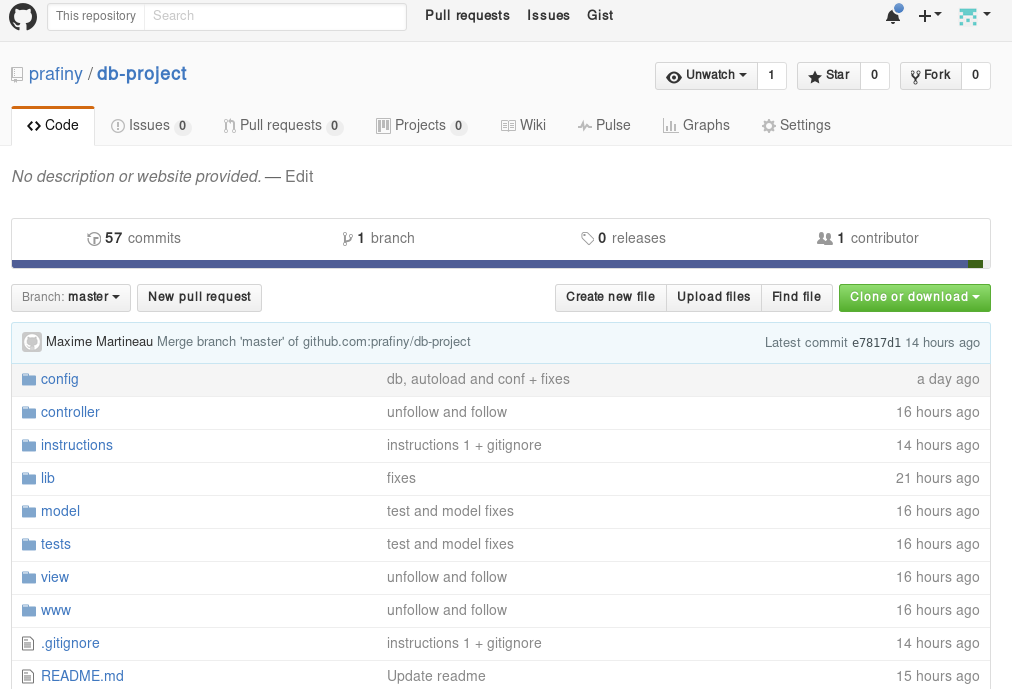
\includegraphics[scale=0.2]{images/project.png}  
\end{frame}

\begin{frame}{Code}
    \begin{center}
        %\url{http://github.com/prafiny/db-project}
    \end{center}

\begin{enumerate}

\item Application can be run in browser (see instructions)
\item Unit tests can be run to check the functions (see instructions)
\item Instructions (in the folder \texttt{instructions/})
\item DB schemas in \texttt{sql/schemas.sql} and entries in \texttt{sql/entries.sql}
\item The goal is to fill out the models (files in folder \texttt{model\_student/})
\begin{enumerate}
\item Read 0setup.pdf for environment installation
\item Read 1user.pdf for first work
\end{enumerate}
\end{enumerate}

\end{frame}

\end{document}


